% This project is a template slides for the subsequent presentations which are significant during the postgraduate period.
% Template for College of Information Science and Electronic Engineering, Zhejiang University.
% Compiled with pdflatex.
% By Xue Shengke.

\documentclass[16pt]{beamer}	% font and size
\mode<presentation>
{
	%\setbeamercovered{dynamic}	% translucent when using pause
	\setbeamertemplate{navigation symbols}{}	% hide navigation bars
	%\setbeamertemplate{caption}[numbered]	% numerate captions
	\setbeamertemplate{background}{
\includegraphics[height=\paperheight]{norm.pdf}}	% set background image
%	\setbeamertemplate{footline}{\textcolor{light-gray}{\scriptsize \insertframenumber/\inserttotalframenumber} \hfill}	% display page number at bottom left corner	
}

%\usepackage{CJKutf8}	% encode for Chinese
\usepackage{times}		% font for english, Times New Roman
\usepackage{amsmath, amsfonts, amssymb}	% math equations, symbols
\usepackage{times}
\usepackage[english]{babel}
\usepackage{xcolor}		% color content
\usepackage{graphicx}	% import figures
\usepackage{url}		% hyperlinks
\usepackage{bm}			% bold type for equations
\usepackage{hyperref}	% bookmarks
%\hypersetup{bookmarks, unicode}	% unicode
\usepackage{listings}
\usepackage{ctex}
\newcommand{\ftitle}[1]{\frametitle{#1}}	% userdefine frametitle
\definecolor{light-gray}{gray}{1.10}
\definecolor{myTitleColor}{RGB}{0,102,204}  % 自定义颜色
\definecolor{mySectionColor}{RGB}{0,0,0}  % 自定义颜色
\setbeamercolor{title}{fg=myTitleColor}  % 设置标题颜色
\setbeamercolor{frametitle}{fg=myTitleColor} 
\setbeamercolor{section in toc}{fg=mySectionColor}  % 设置目录中章节标题颜
\setbeamercolor{block title}{fg=myTitleColor} 
\lstset{
backgroundcolor=\color{white},      % choose the background color
basicstyle=\footnotesize\ttfamily,  % size of fonts used for the code
columns=fullflexible,
tabsize=8,
numbers=none, 
breaklines=true,               % automatic line breaking only at whitespace
captionpos=b,                  % sets the caption-position to bottom
escapeinside={\%*}{*)},        % if you want to add LaTeX within your code
keywordstyle=\color{blue},     % keyword style
%stringstyle=\color{mymauve}\ttfamily,  % string literal style
frame=none,
rulesepcolor=\color{red!20!green!20!blue!20},
% identifierstyle=\color{red},
language=c++,
}
\begin{document}
%	\begin{CJK}{UTF8}{song}	% all Chinese should be enclosed between the commands
		
		\title{\huge 物联网小组汇报}
		\author{杨智晨,周磊,陈坤,邵继诚}
		\institute[NUIST]{\normalsize 
			
\includegraphics[width=0.2\linewidth]{pic/nuist_logo.eps}  \\  % add a special logo on cover page
			School of Electronics \& Information Engineering \\
			%电子与信息工程学院 \\
			NUIST \\
			%南京信息工程大学
		}
		\date{Fall , 2024}
		
		\begin{frame}
			\titlepage	% make the cover page here
		\end{frame}
		
	%	\begin{frame}{Content 目录}
	%		\tableofcontents[sectionstyle=show,subsectionstyle=show/shaded/hide,subsubsectionstyle=show/shaded/hide]
	%	\end{frame}
		\AtBeginSection[]
		{
			\begin{frame}
				\ftitle{Content 目录}		% contents for better review
			\tableofcontents[currentsection, currentsubsection]
	    	\end{frame}
	    }
		
	
		
		\section{1.简单的介绍}
		\begin{frame}
			\ftitle{1.简单的介绍}
			本次项目是一个基于esp8266的物联网点阵时钟。\\ \hspace*{\fill}
		\small	\\项目地址:https://gitee.com/lengff/esp8266-lattice-clock-open
			\\博客地址:http://blog.lengff.com/2022/01/17/project-lattice-clock/
		\\ \hspace*{\fill} \\	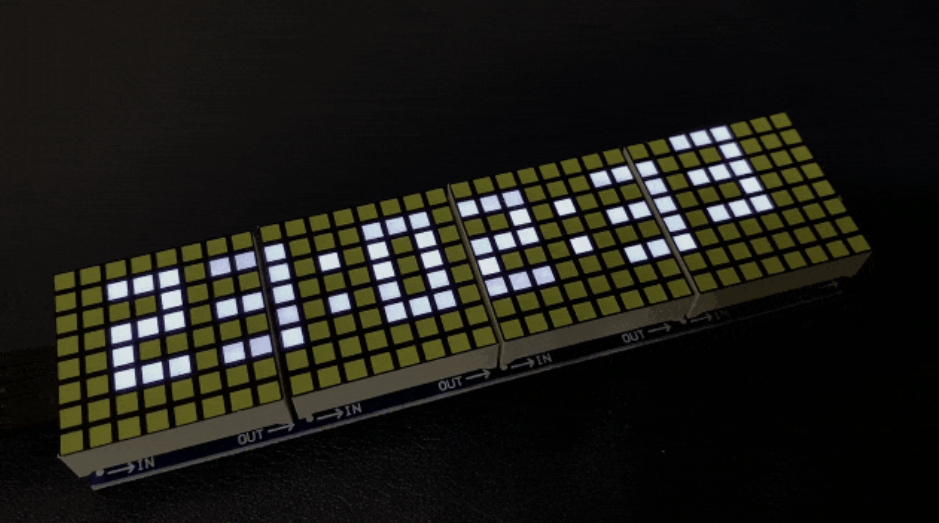
\includegraphics[width=0.8\textwidth]{pic/1-1.png}
		\end{frame}
		\begin{frame}
			\begin{block}{硬件选材}
			\small NodeMcu(Esp8266)\\DS3231\\Max7219 32x8 点阵\\单路触摸模块
			\end{block}
			\begin{block}{主要功能}
			\small	NTP校时
				\\调节显示方向
				\\息屏
				\\调节亮度
				\\显示时间
				\\显示日期
				\\显示倒计时
				\\显示温度
				\\显示B站粉丝数
				\\显示自定义内容
				\\OTA更新
				\\热点模式
			\end{block}
		\end{frame}
		
		\section{2.esp8266联网\&自定义UDP}
		\begin{frame}
			\ftitle{2.esp8266联网\&自定义UDP}
		一、UDP介绍:
	    \\ \hspace*{\fill} \\UDP(User Datagram Protocol)——  用户数据报协议,是互联网传输层的一个重要协议。
		特点:无连接、尽最大努力交付、面向数据报的,首部开销小,概率丢包。
		\\ \hspace*{\fill} \\\centering 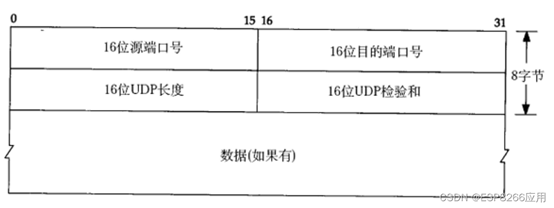
\includegraphics[width=0.8\textwidth]{pic/2-1.png}
		\end{frame}
		\begin{frame}
		二、自定义UDP协议
			\\  \centering 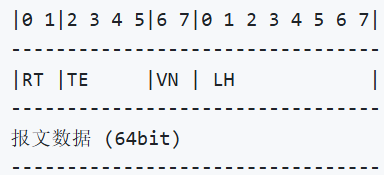
\includegraphics[width=0.8\textwidth]{pic/2-2.png}
			\begin{flushleft}
			1. RT: (2bit)成功返回数值
			\\2. TE: (4bit)type报文类型: 0: 重置时间 ,1: 设置亮度 ,2: 切换功能 ,3: 切换功能显示样式 ,4: 订阅BIlibiliUID ,5: 是否启用点阵屏幕 ,6: 切换显示方向 ,7: 设置用户数据 ,8: 设置动画速度 ,9: OTA 升级 10:设置倒计时 11:设置睡眠时间
			\\3. VN: (2bit)version协议版本,目前固定为1
			\\4. LH: (8bit)length数据包长度
			\\5. 报文数据: (64)bit 版本1目前支持的最大数据包长度为64bit
	    	\end{flushleft}
		\end{frame}
	
		\begin{frame}[fragile]
		三、建立自定义UDP传输和处理流程
		\\ \hspace*{\fill} \\1、引入库文件、创建UDP对象
\begin{lstlisting}
<ESP8266WiFi.h>
<WiFiUdp.h>
WiFiUDP udp;
\end{lstlisting}
		\\ \hspace*{\fill} \\WiFiUdp.h 的作用:	\\ \hspace*{\fill} \\
		\begin{small}
		\\封装 UDP 协议:\\WiFiUdp 类提供了封装好的 UDP 协议函数,允许在应用层发送和接收数据包,库函数自动处理 UDP 协议的封装和解析。
		\\基于 WiFi 连接:\\在使用这些函数之前,需要确保设备已经连接到 WiFi 网络。
	    \end{small}
	    \end{frame}
	    \begin{frame}[fragile]
	    2、Wifi配置连接
	   \\ \hspace*{\fill} \\ \small 1)STA(Station)模式
\begin{lstlisting}
WiFi.mode(WIFI_STA);
WiFi.begin(WiFi.SSID().c_str(), WiFi.psk().c_str()); 
\end{lstlisting}
\\ 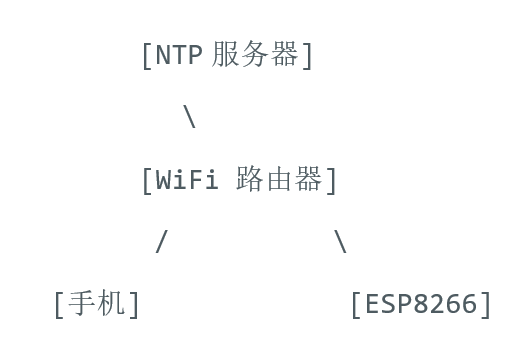
\includegraphics[width=0.6\textwidth]{pic/2-3.png}
\\在STA模式下,esp8266作为wifi网络的客户端接入路由器,与该路由器连接的手机和esp8266处于同一局域网,手机发送指令,esp8266接受并执行对应操作。
	    \end{frame}
	    \begin{frame}[fragile]
	  \small  此外,在STA模式下,esp8266可以通过网络访问NTP服务器进行时间校正
	\begin{lstlisting}
const char *ntpServerName = ''cn.ntp.org.cn'';  //NTP域名
WiFi.hostByName(ntpServerName, timeServerIP);
                                      //将域名转换成IP地址
udp.begin(localPort); // 启动监听本地端口
发送NTP请求
memset(packetBuffer, 0, NTP\_PACKET\_SIZE); 
                                   // 将字节数组初始化为0
packetBuffer[0] = 0b11100011;                 //具体请看参考请求报文说明
udp.beginPacket(timeServerIP, remoteNtpPort); 
                               // 配置远端ip地址和端口
udp.write(packetBuffer, NTP\_PACKET\_SIZE);     // 发送数据
udp.endPacket();                              // 结束发送数据
获取NTP时间戳
int packetSize = udp.parsePacket();//解析数据包,非空为1
if (packetSize) {
udp.read(packetBuffer, NTP\_PACKET\_SIZE);}
                    //解析UDP数据包中的数据到packetBuffer中
\end{lstlisting}
\small NTP(Network Time Protocol),网络时间协议,基于UDP报文进行传输,可以对网络内所有具有时钟的设备进行时钟同步,使网络内所有设备的时钟保持一致,从而使设备能够提供基于统一时间的多种应用。
	  \end{frame}
	    \begin{frame}[fragile]
	  	\small  2)AP模式(热点模式)
	  	\begin{lstlisting}
WiFi.mode(WIFI\_AP\_STA);                  // 同时支持STA和AP
WiFi.softAPConfig(apIP, apIP, IPAddress(255, 255, 255, 0)); //配置AP IP地址
WiFi.softAP(AP\_NAME, NULL, 1, 0, 4);            //设置AP SSID  
\end{lstlisting}
	\centering 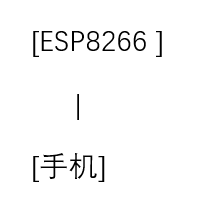
\includegraphics[width=0.2\textwidth]{pic/2-4.png}
	 \begin{flushleft} \small 在AP模式下,ESP8266 会创建自己的 WiFi 热点,手机直接连接到 ESP8266 的 WiFi 热点,不需要连接任何外部网络
	 \end{flushleft}
	 \end{frame}
	   \begin{frame}[fragile]
	 	3、自定义 UDP 数据接收与处理
\begin{lstlisting}
Udpdata Udps::userLatticeLoop(uint8_t power, uint8_t mode, uint8_t version)
\end{lstlisting}
\small 1)通过 parsePacket() 检查是否有 UDP 数据包,若有则读取到缓冲区packetBuffer并处理
\\2)根据数据包版本信息和返回类型构造相应的应答包,暂存缓冲区replyPacket,发送给原先发来的远程主机 udp.beginPacket(udp.remoteIP(), udp.remotePort()); 
\\3)缓冲区packetBuffer数据对应存放到结构体数据udpdata,并作为函数返回值
\begin{lstlisting}
struct Udpdata{
uint8\_t rt;       // 返回类型
uint8\_t te;       // 数据类型
uint8\_t lh;       // 数据长度
uint8\_t data[64]; // 数据包
};
\end{lstlisting}
\small 结构体定义不必和自定义协议一致,很明显少了VN(版本信息)
	 \end{frame}
	 \begin{frame}
		\centering 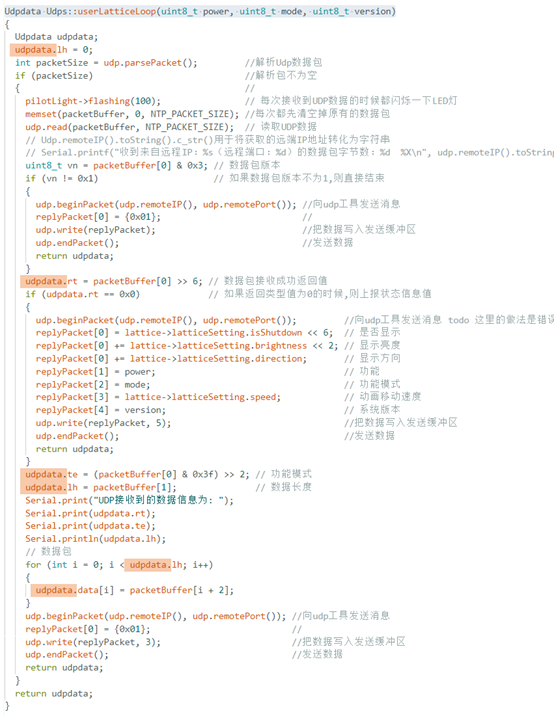
\includegraphics[height=\paperheight]{pic/2-5.png} 
	 \end{frame}
	  \begin{frame}
	 	4、根据接受的UDP数据udpdata.te(报文类型)执行相应操作
	 		\centering 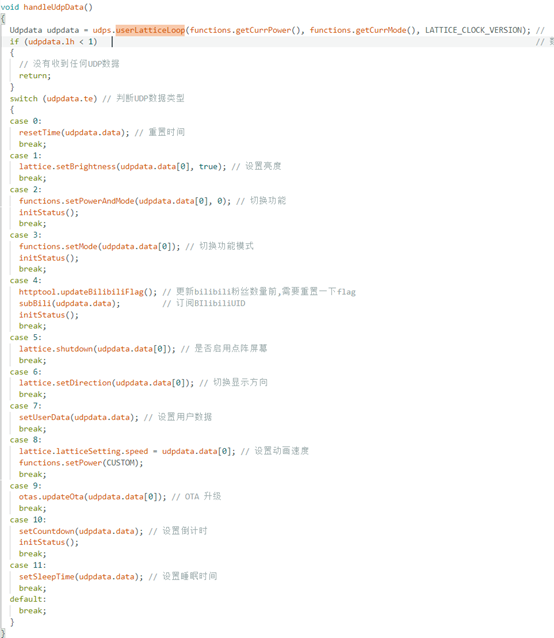
\includegraphics[height=\paperheight]{pic/2-6.png} 
	 \end{frame}
		
		\section{3.微信小程序}
		\begin{frame}
			\ftitle{3.微信小程序}
	\small	1、微信小程序功能	\\ \hspace*{\fill} 
	\scriptsize	\\同步设备状态:设备状态包括什么信息,如何实时同步?是否有状态反馈机制?哪些状态对用户操作有指导意义?
		\\设置显示方向:用户可以通过小程序调整点阵时钟的显示方向,以适应不同安装环境。你可以详细解释如何通过小程序发送方向设置信号,ESP8266如何接收到并处理该信号来实现屏幕旋转。
		\\设置亮度:说明亮度调节的意义,比如在不同环境下调整亮度如何提升用户体验。此外,可以描述亮度调节的范围、精度以及对电量的影响。
		\\切换显示内容:可以介绍该功能支持显示的内容类型(时间、日期、温度等)以及数据来源,如何通过小程序与ESP8266通信来更改显示的内容。
		\\切换显示模式:介绍不同的显示模式(如静态显示、滚动显示等)之间的切换逻辑,以及其应用场景。
		\\恢复出厂:描述恢复出厂设置的用途,如何确保设备在出现故障时能够重置为默认状态,并确保用户操作的简单性。
		\\WiFi配网和热点模式:解释如何通过小程序进行WiFi配网,热点模式下的使用场景(如无WiFi环境时的临时使用),以及这两个模式对设备联网体验的提升。
		\\倒计时设置:扩展说明倒计时功能的用途,如在厨房计时、学习计时等场景中的应用。
		\\OTA更新:详细说明如何通过微信小程序实现远程固件更新,以保持设备软件的最新状态,确保安全性和功能性。\\自定义点阵内容:进一步解释用户可以如何通过小程序自定义显示内容,比如输入文本、设计图案等,并提到内容的最大限制(如字符数、图案复杂度)。
		\end{frame}
		\begin{frame}
			\small	2、为什么会选择小程序来和Esp8266交互呢?	\\ \hspace*{\fill} 
			\scriptsize	\\开发便捷:小程序的开发成本较低,不需要用户安装繁重的APP,依托微信生态,用户获取和使用更为方便。同时可以调动微信提供的多种API(如网络、位置、支付等),扩展了功能实现的可能性。
			\\用户体验:简化交互,节省学习成本,用户只需通过微信小程序即可轻松控制设备,无需学习复杂的操作步骤,适合更广泛的用户群体。
			\\跨平台支持:微信小程序可以在不同的操作系统(如iOS和Android)上无缝运行,而不需要针对不同平台开发独立的应用,节省了开发和维护成本。
			\\丰富的功能支持:如你提到的,微信小程序支持的功能包括WiFi配网、UDP通信、蓝牙等,扩展了设备的操作范围。
		\end{frame}
		\begin{frame}
			\small 3、页面展示:\\ \hspace*{\fill} \\
			 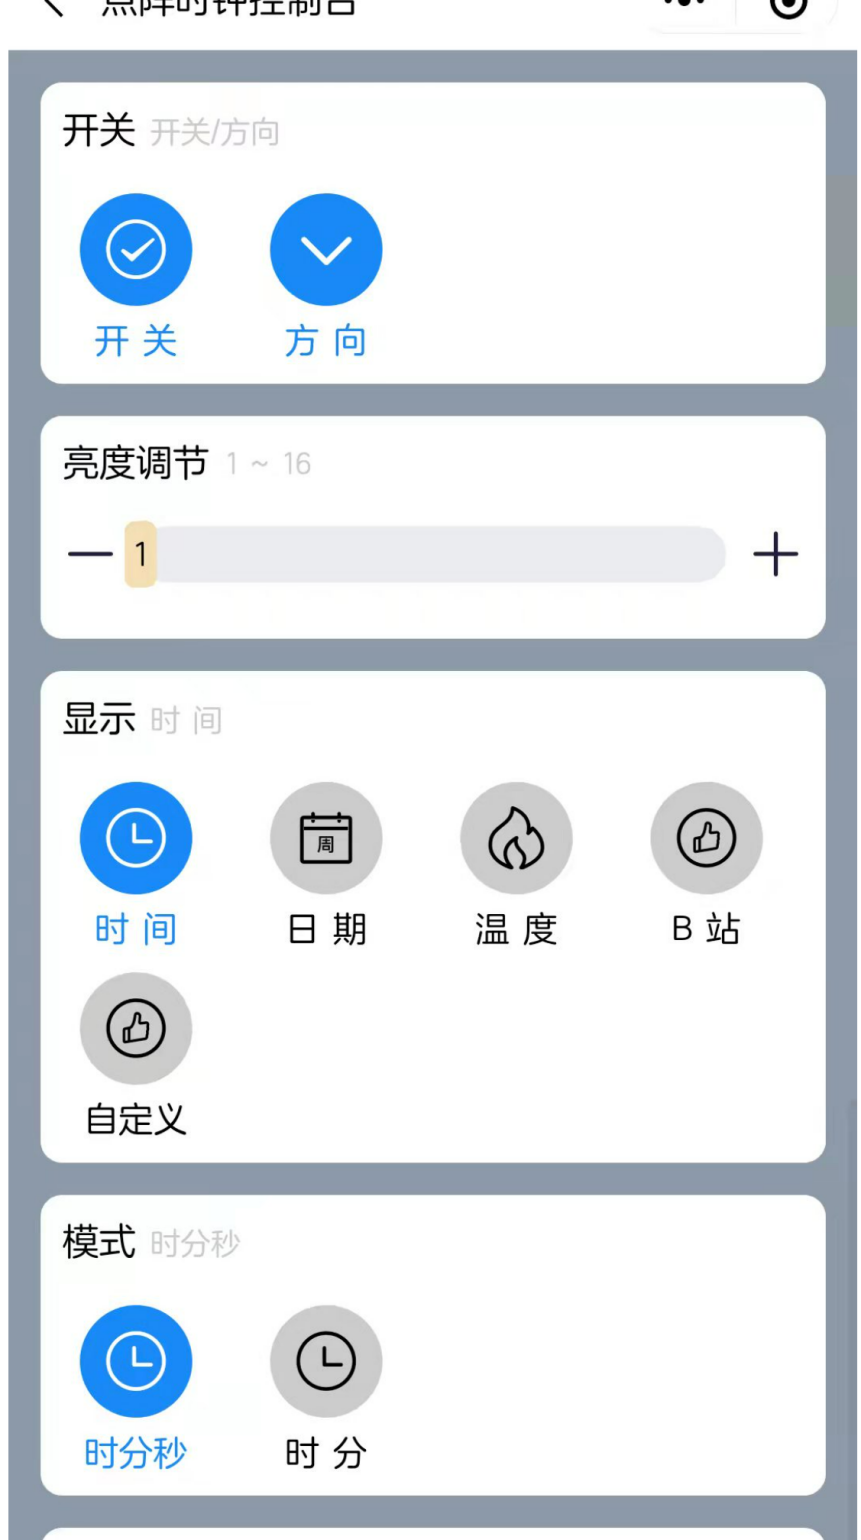
\includegraphics[width=0.3\textwidth]{pic/3-1.png}           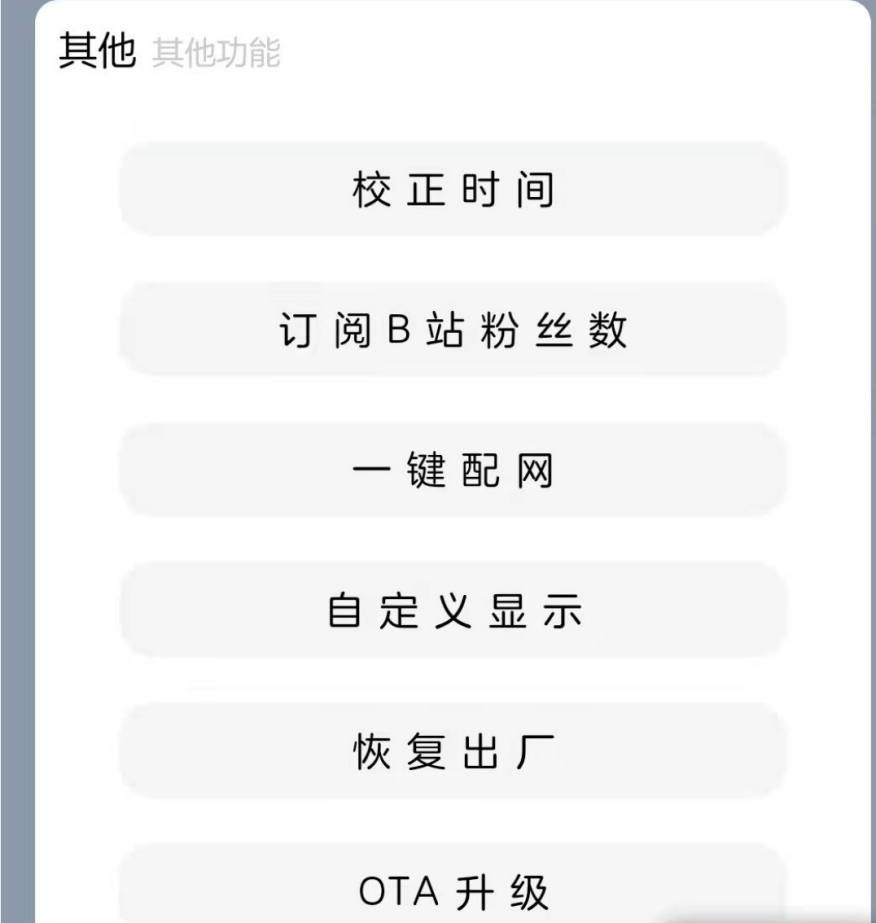
\includegraphics[width=0.5\textwidth]{pic/3-2.png} 
		\end{frame}
		\begin{frame}
			\small4、通讯方式:	\\ \hspace*{\fill} 
			\scriptsize	\\ UDP的特点:UDP是一种无连接的通信协议,简单易用,数据传输速度快,但缺少确认机制,可能会发生数据包丢失或乱序。可以介绍如何权衡速度和稳定性,以及为什么UDP在物联网场景下是合适的选择。
			\\UDP的优缺点:详细说明它的优点,如无需建立连接、广播发现设备,适用于本地网络中的低时延场景。缺点方面,可以扩展如何缓解丢包问题,例如你提到的重复发送指令机制,是否还有其他方法如增加校验码或重传机制。
			\\实际应用中UDP的表现:讨论实际测试过程中UDP通信的表现,遇到的挑战,以及如何在未来版本中通过改进通信协议或引入容错机制来优化通信效果。
			\\ \hspace*{\fill} \\ 
\includegraphics[width=0.5\textwidth]{pic/3-3.png}
			\\这是小程序入口,可以通过手机微信扫描上面的小程序码。
		\end{frame}
		\begin{frame}
		\small 	5、成品图\\ \hspace*{\fill}
		\\ 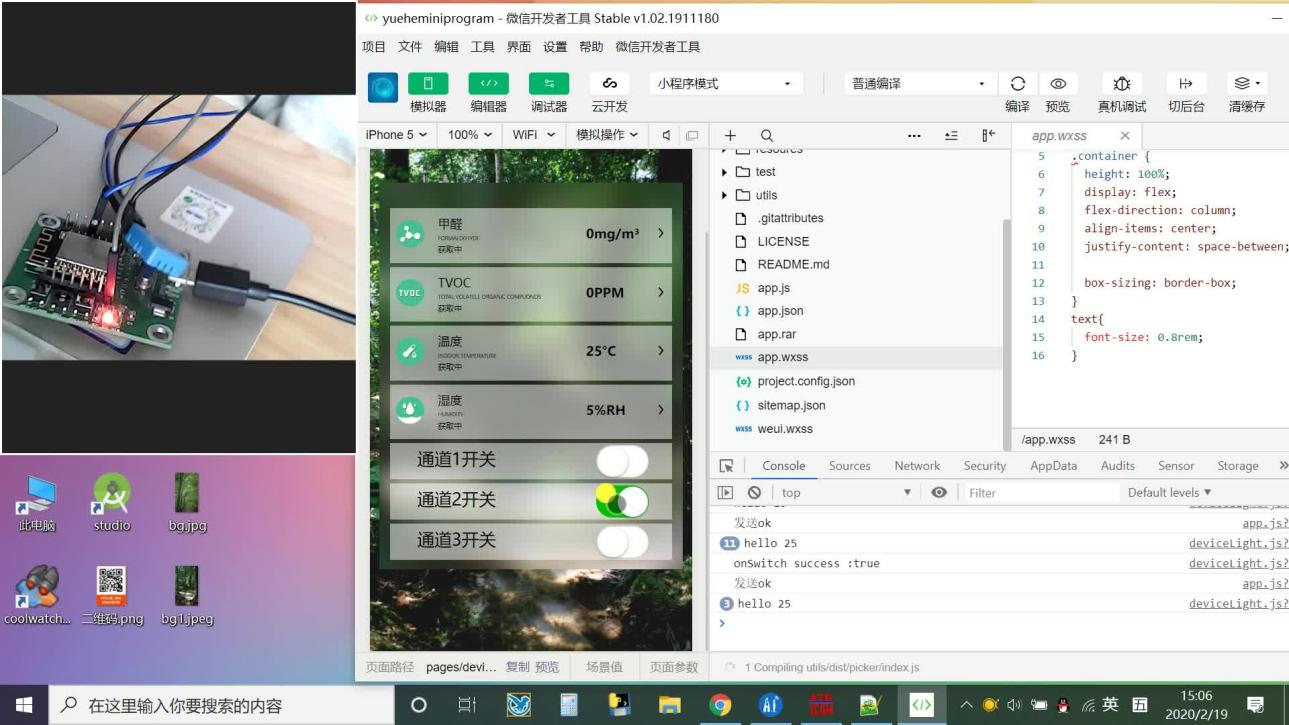
\includegraphics[width=1.0\textwidth]{pic/3-4.png}
		\end{frame}
		
		\section{4.blinker}
		\begin{frame}
			\ftitle{4.blinker}
			采用的控制器是点灯科技的一个app——blinker\\ \hspace*{\fill} \\
			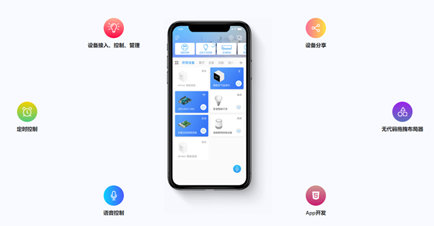
\includegraphics[width=0.8\textwidth]{pic/4-1.png}
	    \end{frame}	
		\begin{frame}
		该app能支持的设备很多,除了一些独立设备,还包括一些现成的其他品牌的产品,如热水器、感应灯、电动窗帘等
		\\ \hspace*{\fill} \\\centering 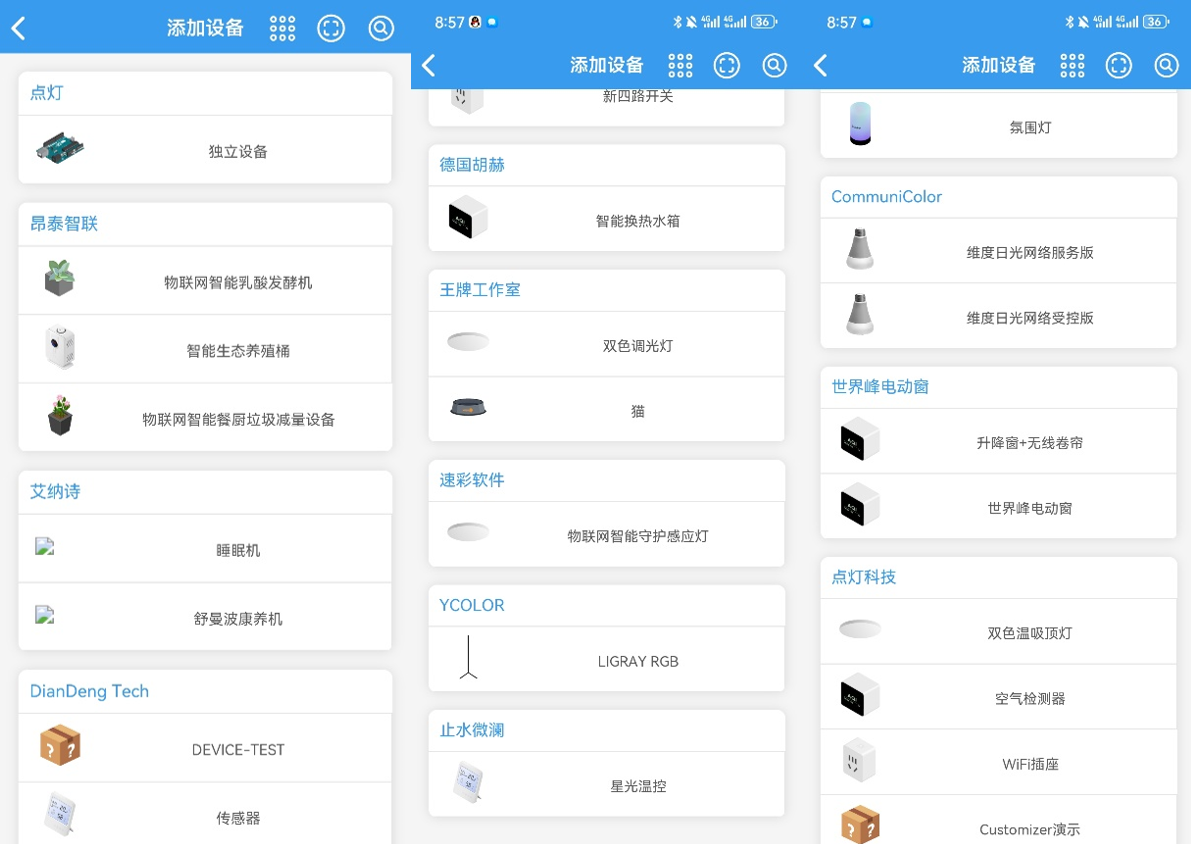
\includegraphics[width=0.8\textwidth]{pic/4-2.png}
        \end{frame}	
	   	\begin{frame}
	    该APP不需要自己配网,直接使用wifi或热点就可以连接设备
	    	\\ \hspace*{\fill} \\\centering 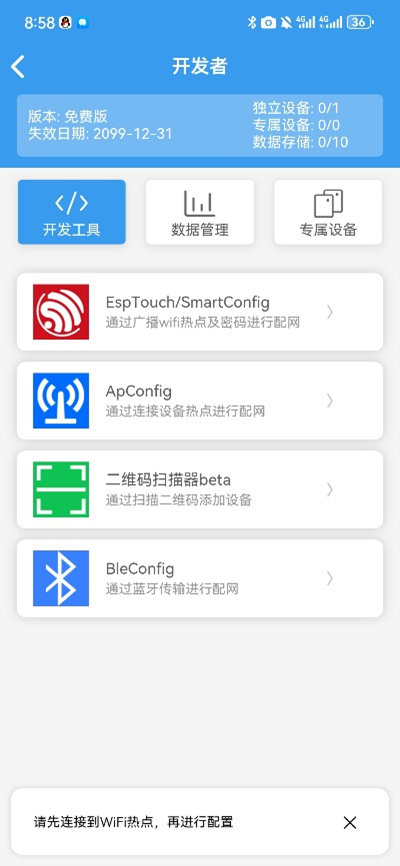
\includegraphics[width=0.3\textwidth]{pic/4-3.png}
	    \end{frame}	
	    \begin{frame}
	    该app提供了设备管理功能和自定义按键功能,且UI设计简洁。
	    例如可以使用区域管理或场景管理来一次性管理同一个区域内或同一个场景下的多台设备,而且他有一个地理视图模式,当设备部署的范围较大时或设备处在移动中时,可以用这个地理视图模式,方便知道设备的位置。
	    	\\ \hspace*{\fill} \\\centering 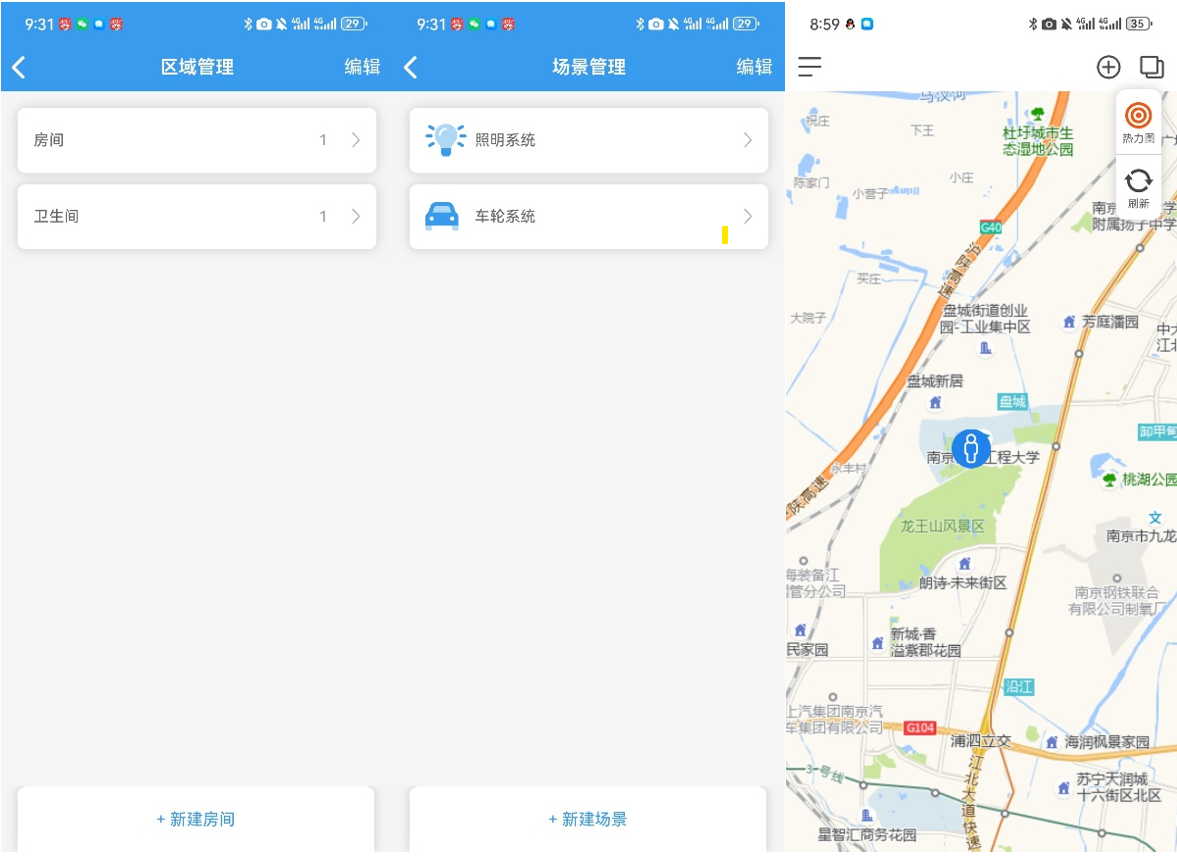
\includegraphics[width=0.8\textwidth]{pic/4-4.png}
	    \end{frame}	
	    \begin{frame}
	    	下面是设备的操控界面,除了基本的串口监视器,它还支持用图表等方式来观察设备的输出;
	    	可以用按键、遥感等操控方式,还包括定时器等辅助操控设备的工具。
	    	\\ \hspace*{\fill} \\\centering 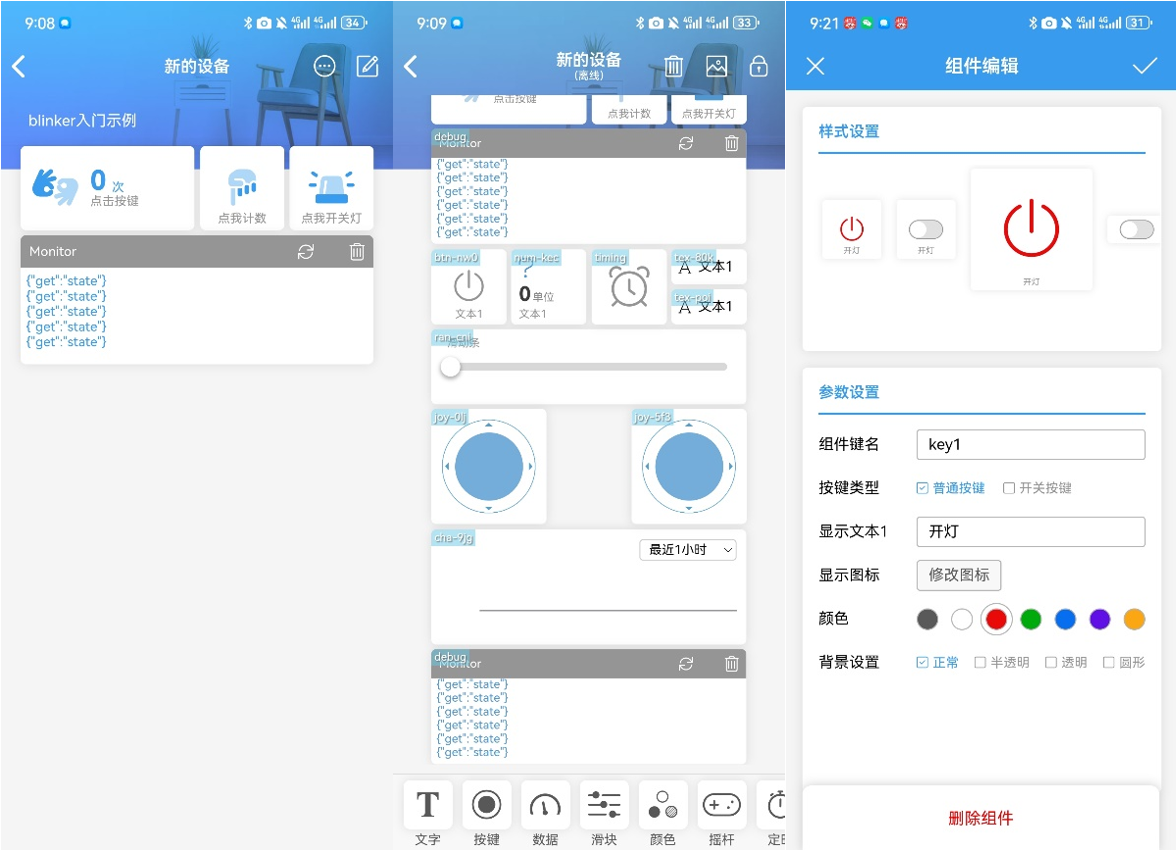
\includegraphics[width=0.8\textwidth]{pic/4-5.png}
	    \end{frame}	
	    
		\section{5.asr}
		\begin{frame}
			\ftitle{5.asr}
			有没有一种可能......
			\\ \hspace*{\fill}	\\ 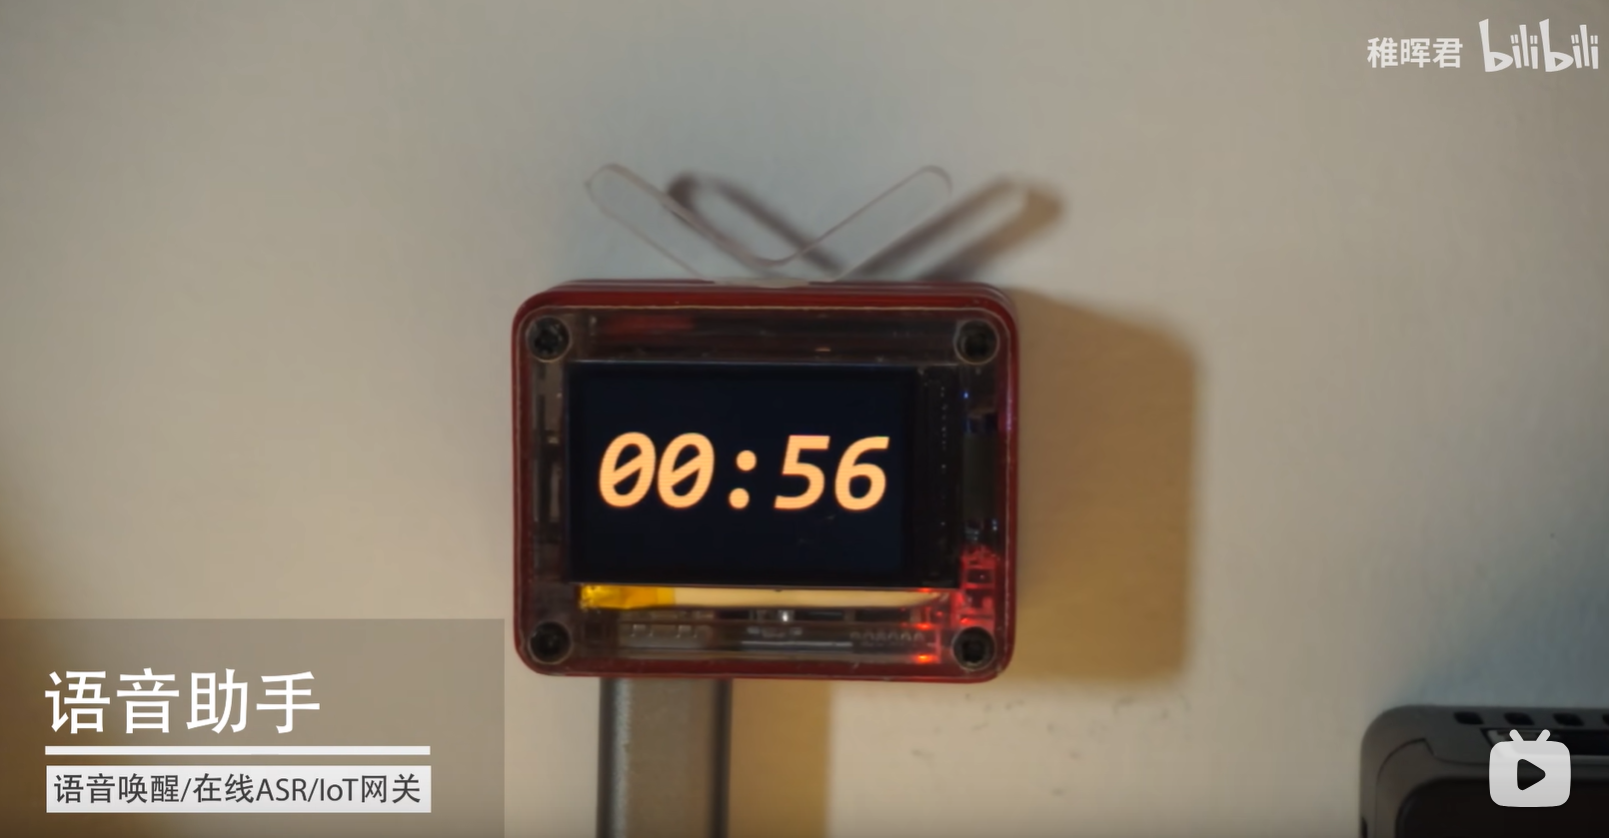
\includegraphics [width=1.0\textwidth]{pic/5-1.png}
		\end{frame}
		\begin{frame}
		  没可能的,辣鸡小艺
		\\ \centering 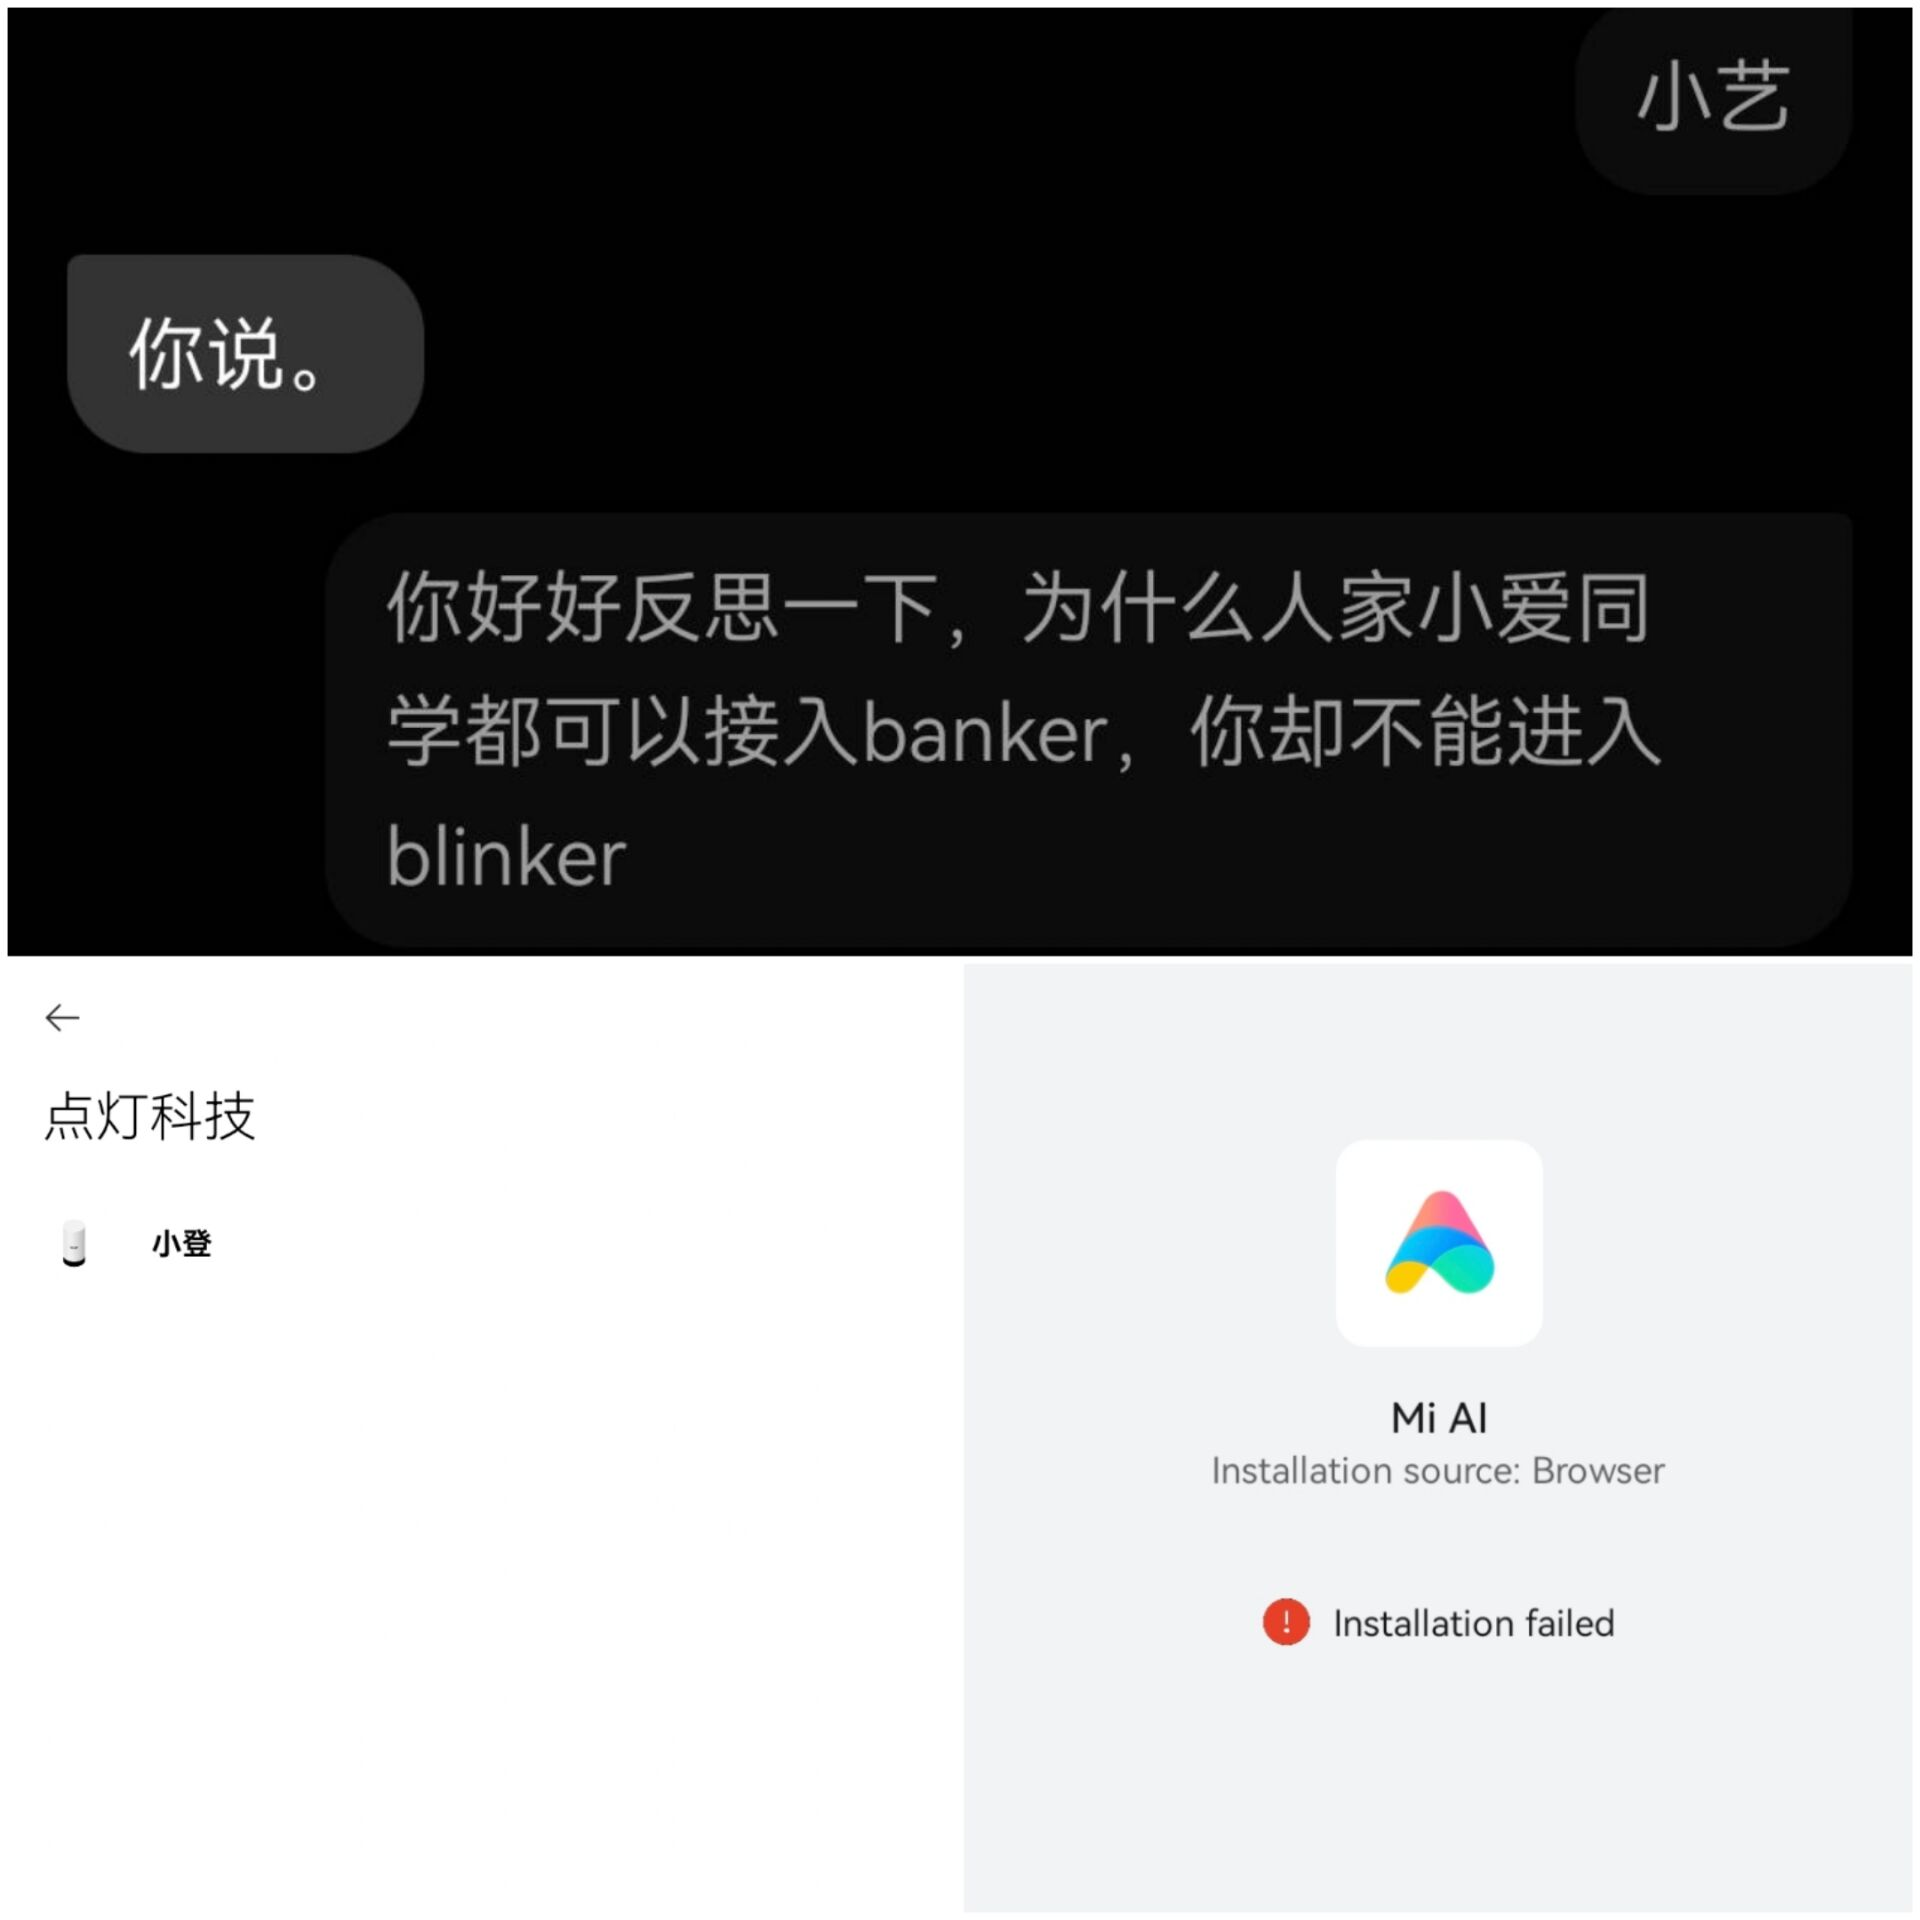
\includegraphics [width=0.8\textwidth]{pic/5-2.jpg}
		\end{frame}
		\begin{frame}
			但是可以试试离线语音模块
			\\项目地址:https://github.com/DIYSmartHome8/Asrpro-ESP8266
			\\天问离线语音模块ASRPro接入Homeassistant
			\\ \centering 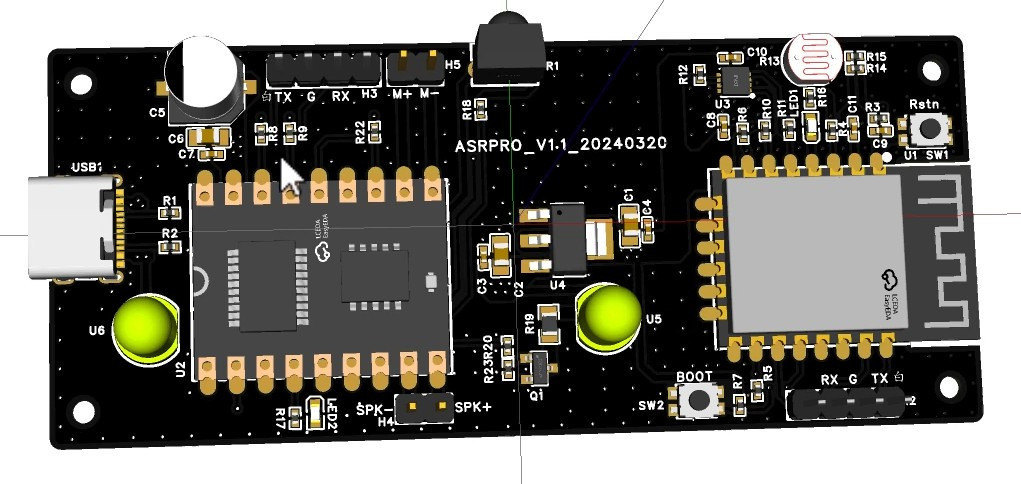
\includegraphics [width=0.8\textwidth]{pic/5-3.jpg}
		 \end{frame}
		 \begin{frame}
		  编写程序使用的天问block,拖拖拽拽,简单
		  \\\centering 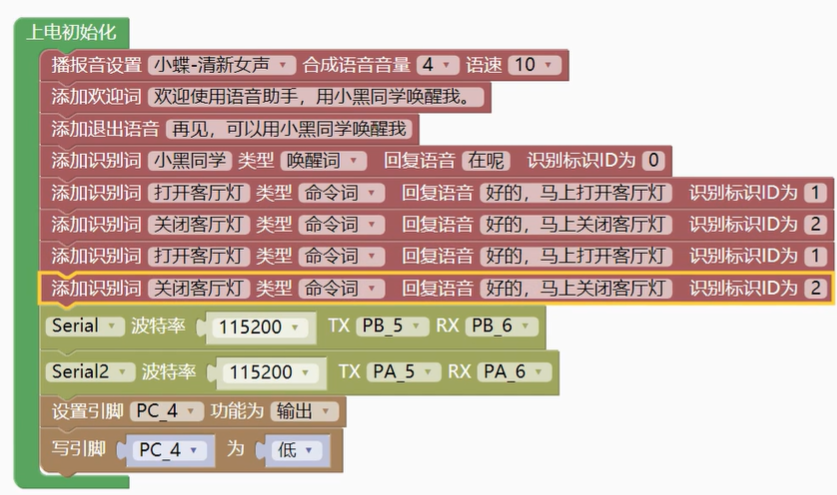
\includegraphics [width=0.8\textwidth]{pic/5-4.png}
		 \end{frame}
		 \begin{frame}
		 	它能做到什么......
		 	\\\hfill\\ 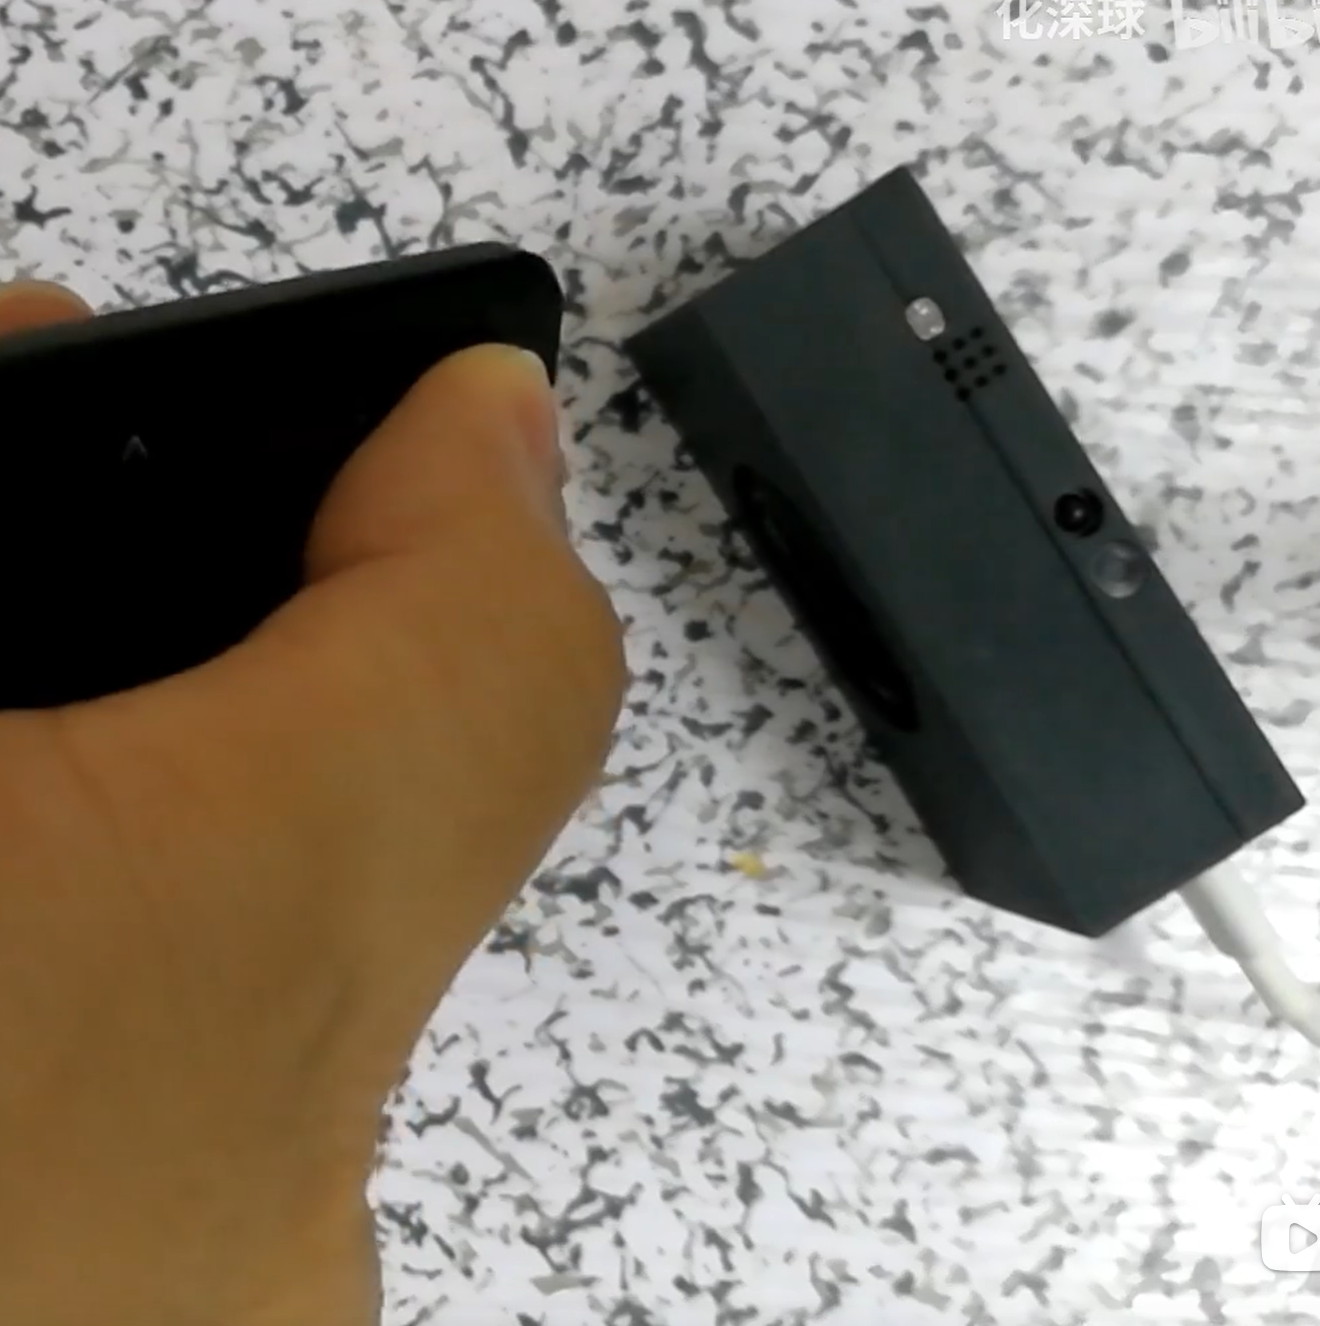
\includegraphics [height=0.6\paperheight]{pic/5-5.png}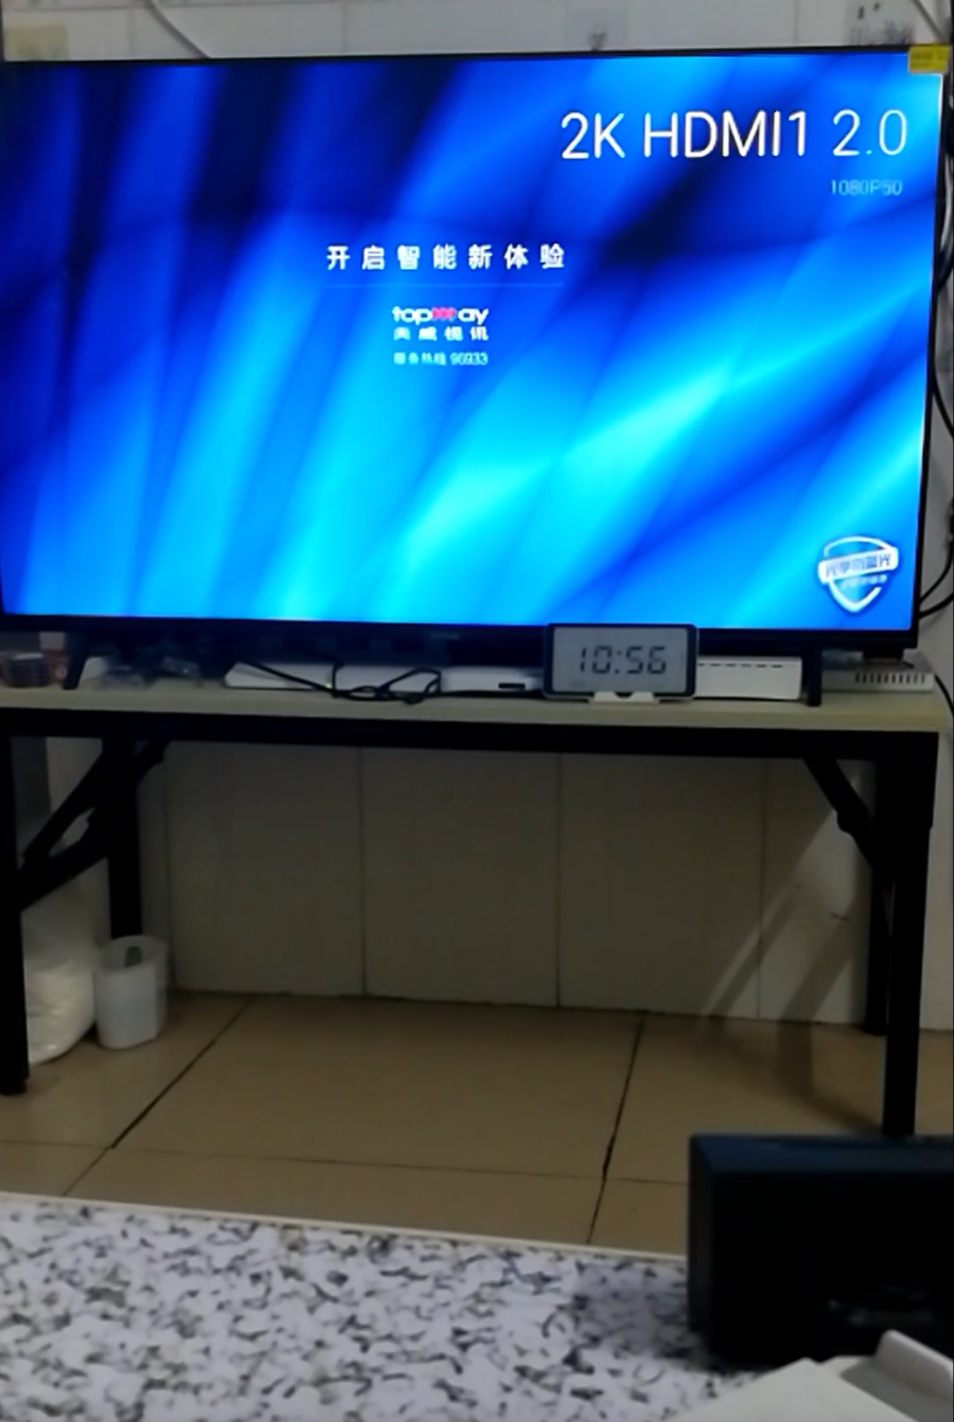
\includegraphics [height=0.6\paperheight]{pic/5-6.png}
		 \end{frame}

\begin{frame}
\Large  ppt模板地址:
\\ https://github.com/synchre/IoTgroupReport
\end{frame}

\setbeamertemplate{background}{
\includegraphics[height=\paperheight]{fin.pdf}}
\begin{frame}
\end{frame}

	
		
		
%	\end{CJK}
\end{document}
